%%%%%%%%%%%%%%%%%%%%%%%%%%%%%%%%%%%%%%%%%
% Dictionary
% LaTeX Template
% Version 1.0 (20/12/14)
%
% This template has been downloaded from:
% http://www.LaTeXTemplates.com
%
% Original author:
% Vel (vel@latextemplates.com) inspired by a template by Marc Lavaud
%
% License:
% CC BY-NC-SA 3.0 (http://creativecommons.org/licenses/by-nc-sa/3.0/)
%
%%%%%%%%%%%%%%%%%%%%%%%%%%%%%%%%%%%%%%%%%

%----------------------------------------------------------------------------------------
%	PACKAGES AND OTHER DOCUMENT CONFIGURATIONS
%----------------------------------------------------------------------------------------

\documentclass[10pt,a4paper,twoside]{article} % 10pt font size, A4 paper and two-sided margins

\usepackage[top=3.5cm,bottom=3.5cm,left=3.7cm,right=4.7cm,columnsep=30pt]{geometry} % Document margins and spacings

\usepackage[utf8]{inputenc} % Required for inputting international characters

\usepackage[T1]{fontenc} % Output font encoding for international characters

\usepackage{polyglossia}
\setdefaultlanguage{english}
\setotherlanguages{russian,ukrainian,chinese,turkish,arabic,french,italian,spanish}
\setmainfont{Helvetica} % font book but only system fonts
\newfontfamily\cyrillicfont[Script=Cyrillic]{Helvetica}


\usepackage{fontspec}

% \usepackage[T2A]{fontenc}      % Font encoding for Cyrillic
% \usepackage[utf8]{inputenc}     % Input encoding for UTF-8
% \usepackage[ukrainian]{babel}   % Ukrainian language support

\usepackage{times} % Use the Palatino font

\usepackage{microtype} % Improves spacings

\usepackage{multicol} % Required for splitting text into multiple columns

\usepackage[bf,sf,center]{titlesec} % Required for modifying section titles - bold, sans-serif, centered

\usepackage{fancyhdr} % Required for modifying headers and footers
\fancyhead[L]{\textsf{\rightmark}} % Top left header
\fancyhead[R]{\textsf{\leftmark}} % Top right header
\renewcommand{\headrulewidth}{1.4pt} % Rule under the header
\fancyfoot[C]{\textbf{\textsf{\thepage}}} % Bottom center footer
\renewcommand{\footrulewidth}{1.4pt} % Rule under the footer
\pagestyle{fancy} % Use the custom headers and footers throughout the document

\newcommand{\entry}[4]{\markboth{#1}{#1}\textbf{#1}\ {(#2)}\ \textit{#3}\ $\bullet$\ {#4}}  % Defines the command to print each word on the page, \markboth{}{} prints the first word on the page in the top left header and the last word in the top right

\usepackage{tikz}
\usetikzlibrary{calc} % Optional, but useful for more complex calculations

\usepackage{textcomp}


%----------------------------------------------------------------------------------------

\begin{document}

%----------------------------------------------------------------------------------------
%	TITLE PAGE
%----------------------------------------------------------------------------------------


\begin{titlepage}

\AddToHookNext{shipout/background}{
    \begin{tikzpicture}[remember picture, overlay]
        \node at ($(current page.south) + (0, 8.25cm)$) % Adjust 1cm for desired distance from bottom
            {\centering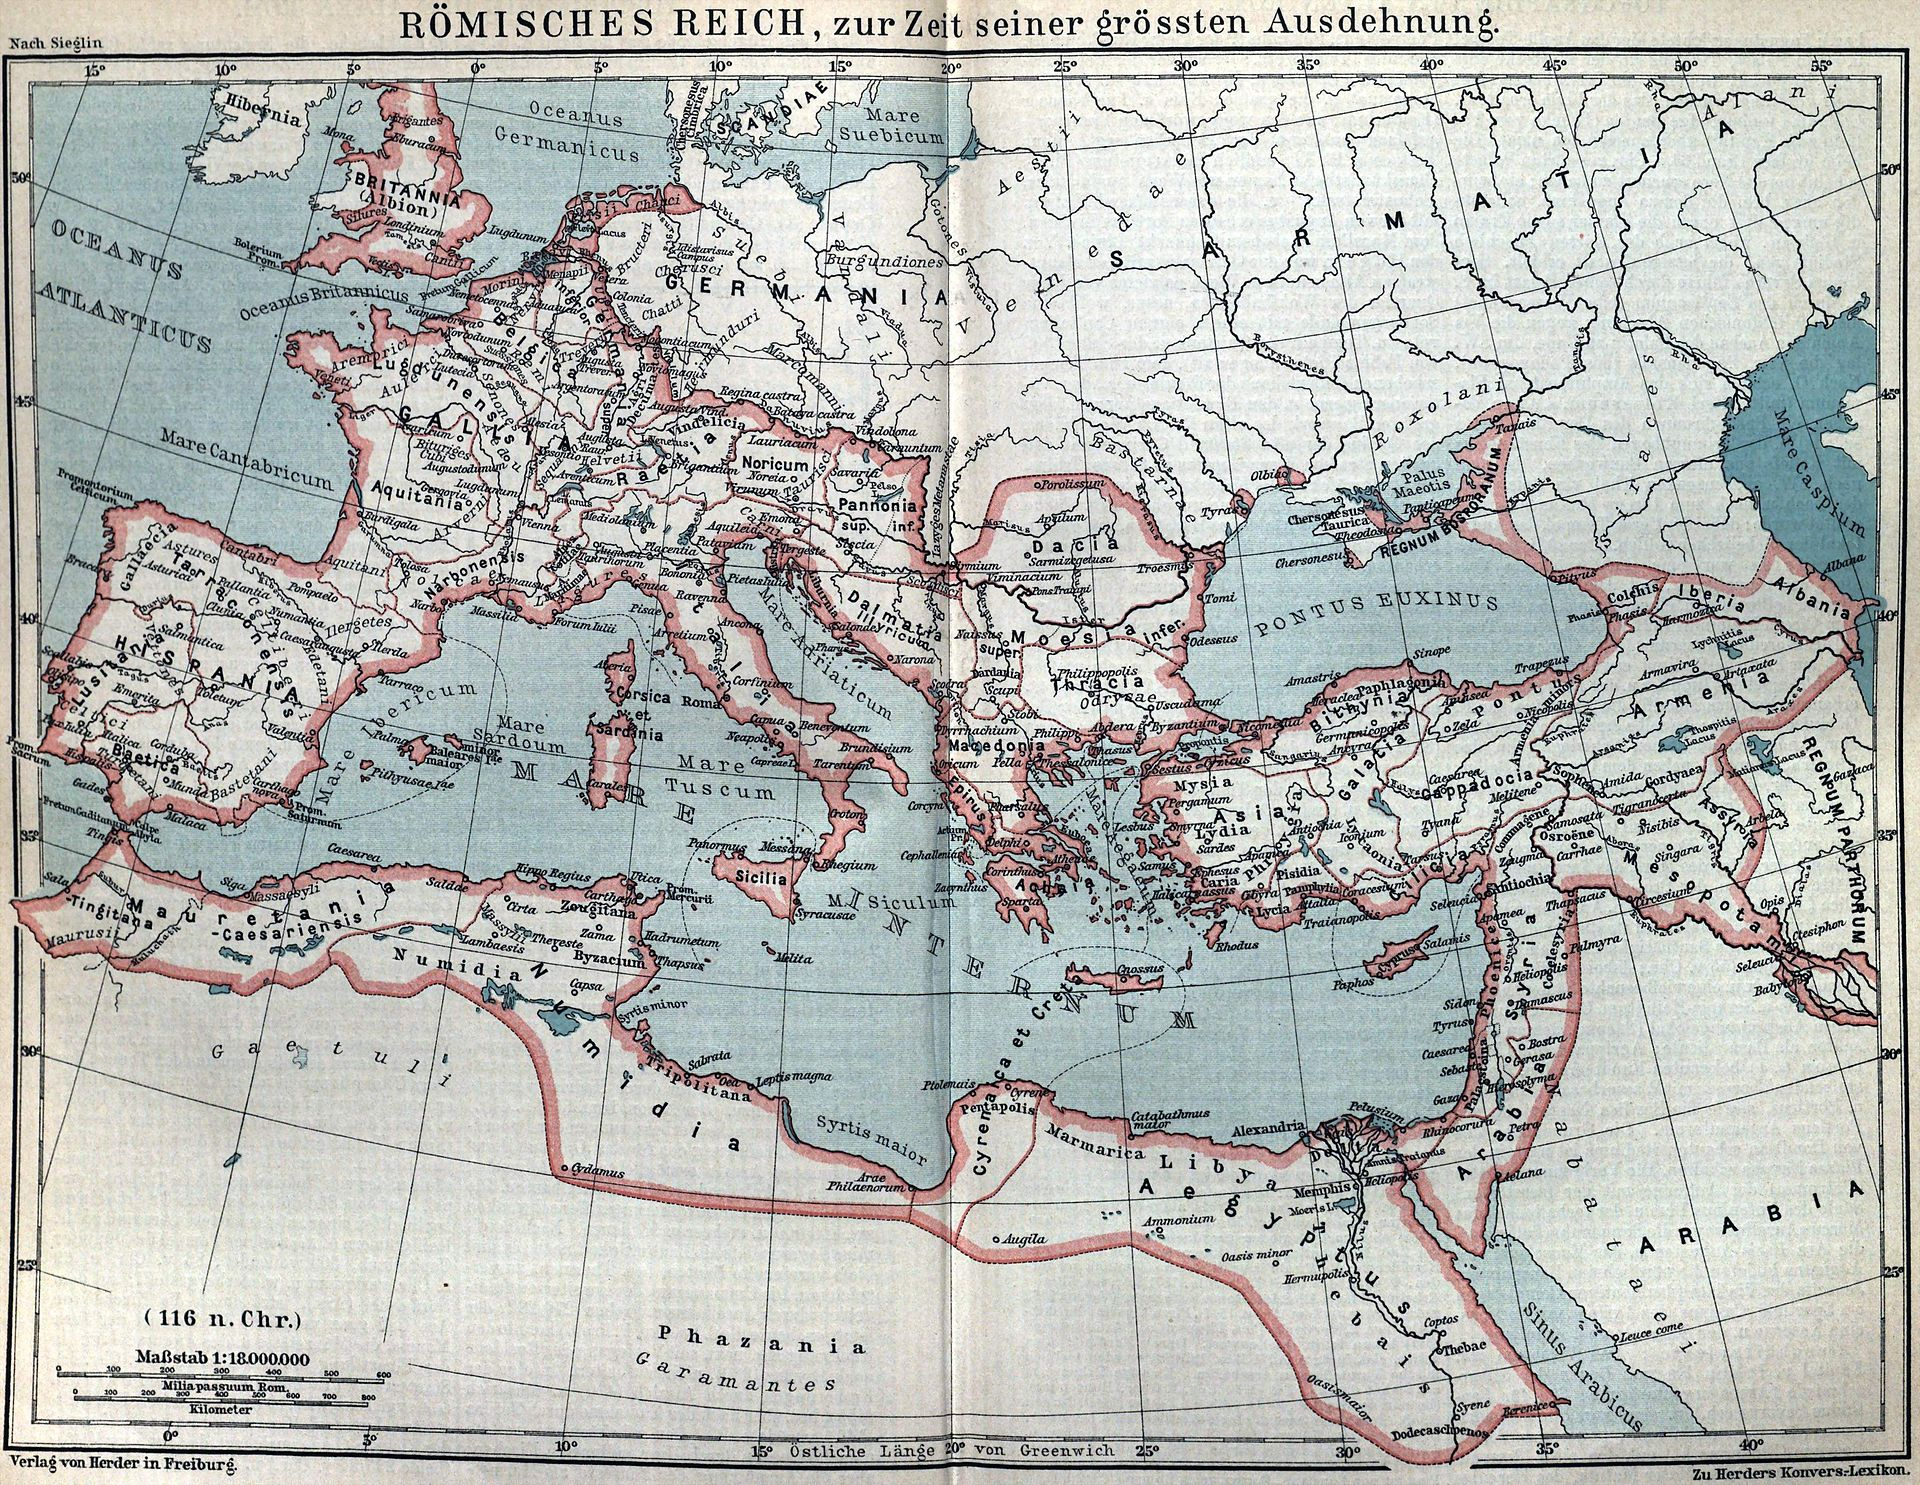
\includegraphics[width=1.5\textwidth]{Regnum_Bosporanum}}; % Adjust width and image filename
    \end{tikzpicture}
}


  \centering % Center all content
    \vspace*{2cm} % Add vertical space from the top
    {\Huge Xersonesus \\} % Large title
    \vspace{1cm}
    {\Large An Historical and Critical Encyclopedia of the Ukraine War \\} % Subtitle
    \vspace{2cm}
    {\Large 3AC3B33B33B53BB3BF3C2 \\} % Author name
    {\normalsize \emph{ seppie coi piselli alla romana } \\}
    \vspace{1cm}
    {\today} % Date
    \vfill % Fill remaining vertical space
    % Add any other elements like logos, disclaimers, etc.


 \end{titlepage}

%----------------------------------------------------------------------------------------
%	SECTION 1
%----------------------------------------------------------------------------------------

\section*{1}

\begin{multicols}{2}

\entry{Artemovsk} {Artemovsk} {Noun} {See \textbf{Bakhmut-Artemovsk}.}

\end{multicols}

%----------------------------------------------------------------------------------------
%	SECTION 2
%----------------------------------------------------------------------------------------

\section*{2}

\begin{multicols}{2}

\entry{2nd Conquerer of Sevastopol} {Artemovsk} {Noun} {See Erich von Manstein.}

\end{multicols}


%----------------------------------------------------------------------------------------
%	SECTION A
%----------------------------------------------------------------------------------------

\section*{A}

\begin{multicols}{2}

\entry{Artemovsk} {Artemovsk} {Noun} {See \textbf{Bakhmut-Artemovsk}.}

\entry{Artillery} {ar·til·ler·y} {Noun} {Coined by the gravedigger of the revolution, Joseph Stalin, artillery is the god of war. The god of war, however, is now but only a vital component in an evolving array of combined arms in eastern Europe. In the beginning of the Ukraine war the  media focused almost exclusively on parity. The number of Russian artillery guns, calibre, the number of munitions, the type of munitions, or the way in which the Russians accurately targeted Ukrainian targets demonstrated the advantage Russia weaned over its opponent.  \newline \indent In the beginning of the Ukraine war, primarily before the great Ukrainian offensive in Kharkiv, launched on September 6th, 2022 but prepared weeks in advance, until the end of Ukraine's 'Spring' counteroffensive in 2023, artillery played a dominant role on the battlefield. Ukraine's failed 'Spring' counteroffensive witnessed confirmed Russia's seizure of the strategic initiative after the fall of Bakhmut-Artemovsk on May 23rd, 2023. In the winter of 2023 the Ukraine war witnessed a major transformation in the deployment of drones. Ukraine began to mass produce First Person View drones to strengthen its defense of the Donbas in the face of continued Russian advances. Necessity is the mother of invention. Ukraine's FPV drones began to play a dominant role on the battlefield, overtaking but by no means substituting for the role artillery played in the beginning of the war. The first Ukrainian brigades with dedicated, trained, expert drone pilots began to take shape.}

\entry{Avdiivka} {} {} {}

\entry{Axe, David} {} {} {One of the more committed journalists of the Ukraine war, whose coverage of the Donbas, especially in the Avdiivka direction from 2023 to the present, eclipsed others. Published primarily in \emph{Forbes}, these articles are an important source of information. At a time when the majority of news from the frontlines comes almost exclusively from 'milbloggers,' Axe's analyses shed light on rarely mentioned or hardly examined aspects of the Ukraine war. \newline \indent \emph{Forbes}, whose annual lists of America's four hundred richest Americans constituted one of the Socialist Equality Party's the primary staples of propaganda in the years preceding the 2008 subprime mortgage crisis, the nine years after the party's launch of the World Socialist Website in 1998\footnote{The SEP's launch preceded the Federal Bureau of Investigation's launch of a Federal Intrusion Detection Network, or FIDNET, modeled after a famous program from Linux's suite of open source security software called Snort, a network intrusion detection system (NIDS). Mentioned in the article published on  August 10th, 1999, under the title "White House plan for FBI Internet spying," FIDNET is one of the earliest precursors to the drag-net surveillance Edward Snowden exposed in his leak of secret documents from the National Security Agency (NSA). Originally exposed in an article published on July 28th, 1999, by the \emph{New York Times} under the title, "The U.S. Drawing Plan That Will Monitor Computer Systems," FIDNET is a part of the pre-history to the U.S. conspiracy to deprive citizens of life, liberty, or the pursuit of happiness through the technological obliteration of the founding father's Bill of Rights, especially the Fourth Amendment. Although the early SEP article makes no mention of the U.S. Constitution, the legal critique would become more apparent as the U.S. conspiracy strengthened its execution.} under the pretense of a Marxian renaissance.\footnote{In an article published on October 31st, 1998 under the title, "International school examines the century’s central problems of history, politics and culture," the International Committee of the Fourth International emphasized how a "central premise guiding the school was that a renaissance of Marxism is fundamental to the development of a perspective that can answer the burning issues of the day—growing social inequality, deepening economic crises, the decline in the cultural level of society and the prevailing political paralysis of the workers movement." } These early articles\footnote{The first appears to be ["Gap between rich and poor is wider than ever," 23 June 1998] but many more follow: ["The Forbes 200 list: billions for the privileged few," June 30, 1999], ["Forbes publishes list of 400 richest Americans," October 6, 2006]. } stand in stark contrast with the present stream of current headlines. It would seem that as opposed to those ten years of doldrums, history's acceleration required expanded coverage, prompting the SEP to abandon its annual review of \emph{Forbes}' lists. \newline \indent Axe's affinity for the representation of events from the Ukraine war in his articles with a relative approximation towards facts, however gained by his ambition for a Ukrainian victory, became a source of unease at the editorial board. Questions like the following likely flashed through \emph{Forbes}'s editorial board: What if an intelligent reader could see through the transparent attempt to portray Ukraine's armed forces in the most positive light imaginable? Might they be able to read between the lines? Wouldn't it be apropos? It would only be a matter of time before \emph{Forbes}, whose aim is to articulate the interest of a wealthy elite, would clash with Axe's propensity for factually based reporting on the highly politicized Ukraine war. \emph{Forbes}, the famous magazine celebrating the top one percent of the nation-state's richest people annually, decided to fire Axe, terminating his coverage before the end of the Ukraine war, the outcome of which has been to deprive posterity of one its auspicious eyes.}

\end{multicols}

%----------------------------------------------------------------------------------------
%	SECTION B
%----------------------------------------------------------------------------------------

\section*{B}

\begin{multicols}{2}

\entry{Bakhmut-Artemovsk} {} {} {The city whose fall sounded a death knell for the Ukrainian strategic initiative. Spellt \textukrainian{Бахмут — Артемівськ} in Ukrainian but —  \textrussian{Бахмут — Артемовск} in Russian, the city's history is unique.  }

\entry{Bombing} {bomb·ing} {Gerund} {Bombing has thus far been ineffective from the beginning of the Ukraine war. It alone has not accomplished a single strategic objective for any of the warring parties. \newline \indent The \emph{New York Times} is one of the most fervent advocates of bombing.\footnote{“How to Choke Iraq,” \emph{NYT}, December 7th, 1990.} \footnote{“Bombing Iraq Ins’t Enough,” \emph{NYT}, January 30th, 1998.} \footnote{“American Bombs Make Iraq Stronger,” \emph{NYT}, December 20th, 1998.} \footnote{“Bomb North Korea, Before It’s Too Late,” \emph{NYT}, April 12th, 2013.} \footnote{“Bomb Syria, Even if It is Illegal,” \emph{NYT}, August 27th, 2013. } \footnote{“To Stop Iran’s Bomb, Bomb Iran,” \emph{NYT}, March 26th, 2015.}

}

\end{multicols}


%----------------------------------------------------------------------------------------
%	SECTION C
%----------------------------------------------------------------------------------------

\section*{C}

\begin{multicols}{2}

\entry{CIA} {Abbreviation} {Noun} {

It is often claimed in print that the CIA (Central Intelligence Agency) predicted the beginning of the Ukraine war. It is true. The CIA forecast Russia's full-scale invasion less than two weeks in advance. \footnote{ It is hard to imagine a time before the \emph{Kyiv Independent}, the newspaper the \emph{Wall Street Journal} tapped to cover the Ukraine war with the immediacy the U.S.-led NATO alliance demands for its rolling propaganda. \textukrainian{\emph{Українська правда}}, however, is one of the few Ukrainian newspapers whose history of publication precedes the struggle for Ukraine. It is thus a newspaper preceding the \emph{Kyiv Independent}'s coverage on the Ukraine war. It published the majority of the articles covering the CIA's predictions. In one of these articles, the headline describes the attack to be within days: \textukrainian{"Байден вважає, що Путін може напасти на Україну в найближчі дні} – The Guardian," \textukrainian{\emph{Українська правда}}, 11 \textukrainian{лютого} 2022. The first of these is reporting on \emph{The Guardian}. It is a reference to the \emph{The Guardian}'s article published on February 11th under the title, "US warns of ‘distinct possibility’ Russia will invade Ukraine within days." Reporting on \emph{Der Spiegel} revealed the date: ["\textukrainian{ЦРУ назвало імовірну дату нападу Росії на Україну} – \emph{Spiegel}," \textukrainian{\emph{Українська правда}}, 11 \textukrainian{Лютого} 2022]. A reference to the \emph{Der Spiegel}'s article published on February 11th under the title, "CIA rechnet mit russischem Angriff kommende Woche," the so-called \textukrainian{імовірна дата} could not have been vague in German. Another published a day after these read: ["\textukrainian{Головні новини п’ятниці та ночі: ймовірний напад Росії, санкції РНБО}, \textukrainian{\emph{Українська правда}}, 12 \textukrainian{Лютого} 2022"].} In the publications in Ukrainian, Hebrew, Russian, or English, the majority of the accompanying images are pulled directly from an article published seven years ahead of its time. On Mar 9, 2015, \emph{Stratfor} published its famous article, "Gaming a Russian Offensive." The scenarios the CIA discusses in its forecast are replications of those from \emph{Stratfor}'s article. The arrows in these sets of images follow those in \emph{Stratfor}'s article.  \newline \indent It is interesting how these new images spiral outward from a common source almost like a Fibonacci sequence, adding more arrows with the fractionalization of the original scenarios.  In one of the articles published by \textukrainian{\emph{Українська правда}}, the newspaper reports on February 12th how \textukrainian{"Росія має 9 маршрутів сэргнення до України, танки можуть сягнути Києва за 2 доби - розвідка США"}. A few of these nine routes, as impractical as the aforementioned fractionalization, could not have been farther from the truth, as the Russia massed scores of Russian troops on the highways into the Donbas, where the majority of the fighting raged for years before Russia launched its full-scale invasion. These three additional scenarios exceed \emph{Stratfor's} original six. 

}

\entry{Cocaine} {drug} {Noun} {Vladimir Putin, the President of the Russian Federation elected by more than 87.8 percent of the vote in Russia's last election in 2024 for a new six year term, becoming Russia's longest-serving leader for more than 200 years, famously declared his preference to work with those whose \textrussian{«Нос в кокаине!»} than \textrussian{«с умными»} in an interview with \textrussian{Димтрий Константинович Киселев} for \textrussian{«России 1»} and \textrussian{РИА Новости} on March 13th, 2024. The reference is in regard to negotiating an end to the Ukraine war. 
\newline \indent Putin claimed that intelligent politicians had by that time started to change strategies for relating to Russia, explaining that these people are dangerous because they want to throw \textrussian{«всякие свои хотелки под видом морковки»} (i.e., ulterior motives under the guise of proposals for a negotiated settlement).\footnote{ [ \textrussian{"Путин рассказал о предпочтении работать с теми, у кого «нос в кокаине»," Газета.ру,  13 марта 2024} ]. } It is therefore to be determined whether the start of serious negotiations for the end of the Ukraine war should start not with a peace proposal but with a mirror, razor or lines of cocaine, is it not? 

}


\end{multicols}


%----------------------------------------------------------------------------------------
%	SECTION D
%----------------------------------------------------------------------------------------

\section*{D}

\begin{multicols}{2}

\entry{Delta} {Title} {Software} {Seldom mentioned in the media, Delta is a battlefield management system preceding the U.S. Army's phased released of its own Large Language Models for AI. Announced by Col. Jonathan Harvey from the U.S. Army on October 18th, 2025, the "sufficient, joint weapon target pairing Large Language Model (LLM)" is scheduled to run inside of the "kill chain," a model advancing from a simple exercise to a "fully devolved reasoning model." The most likely set of data is based on multiple projects running simultaneously in the field of artillery. One of these relates to completing the updates to NATO's firing tables, military artillery data sheets used for calculating trajectories, for the first time since the Cold War.\footnote{["NATO to make fresh push for common arms standards," \emph{Reuters} October 16th, 2024]} Another is likely the collocation of manuals on targeting, tactics, techniques or procedures\footnote{[https://www.cia.gov/readingroom/docs/CIA-RDP07S00452R000300820008-6.pdf]} for field artillery in combination with the aforementioned firing tables. In the face of the revolution the U.S. Army's phased release of its own Large Language Models is expected to achieve for combat management systems, Delta is now a legacy. 
\indent In the first year of the Ukraine war, a Russian affiliated hacker by name of \textrussian{«Джокер»} managed to gain access to a Ukrainian commander's laptop with Delta on or around November 1st, 2022.\footnote{["\textrussian{Безсонов заявил, что хакер из ДНР взломал систему управления войсками ВСУ DELTA},"  \textukrainian{\emph{Известия}}, 1 \textrussian{ноября} 2022], ["\textrussian{Хакер Джокер рассказал подробности о взломе системы управления войсками ВСУ},"  \textukrainian{\emph{Известия}}, 1 \textrussian{ноября} 2022] } Described as a system for controlling Ukrainian troops, the system allegedly contains details about Ukrainian troops. At the time of the \textrussian{Джокер}'s announcement, Delta sounded like an unparalleled Ukrainian advantage in software development for the technology of warfare. In video footage from the article, however, Delta is an interactive map with real time updates. While the video footage is only one glimpse at the program, an interactive map could be hardly anything more than a 'novelty' by the New Year. A trend quickly emerged. The interactive map became a staple among journalists. The Ukrainian 'milblogger', DeepState, associated with Ukraine's intelligence services, championed updates to the "Map of the war in Ukraine," gaining recognition among the world's largest media companies. Military Summary, associated with Russia, is the first channel in the history of warfare to offer daily updates on the frontlines from the beginning of the Ukraine war. These 'mappers' overthrew the interactive maps with news, transforming war coverage forever. 

}


\entry{The Department of Defense} {Title} {Phrase} {In recognition of the role warfare plays in policy, the Trump administration reversed years of intellectually debased stagnation in the U.S. Armed Forces' bureaucracy with the elimination of the Department of Defense for the return of the Department of War during the Ukraine war. 

}

\entry{Donbas} {} {} {}


\end{multicols}

%----------------------------------------------------------------------------------------
%	SECTION E
%----------------------------------------------------------------------------------------

\section*{E}

\begin{multicols}{2}

\entry{Electricity} {} {} {  }

\end{multicols}

%----------------------------------------------------------------------------------------
%	SECTION F
%----------------------------------------------------------------------------------------

\section*{F}

\begin{multicols}{2}

\entry{FAB} {} {} {See "glide kits" (i.e., \textrussian{Унифицированный модуль планирования и коррекции (УМПК))}. }

\end{multicols}

%----------------------------------------------------------------------------------------
%	SECTION G
%----------------------------------------------------------------------------------------

\section*{G}

\begin{multicols}{2}

\entry{Gantz} {} {} {A detailed, thorough, insightful military historian of the eastern front, Gantz is one of the U.S. Army's untapped resources America's intelligence never managed to consult prior to the transformation of Julia Nuland's successful 2014 Maidan \emph{coup d'etat} into a provocation.}

\end{multicols}

%----------------------------------------------------------------------------------------
%	SECTION M
%----------------------------------------------------------------------------------------

\section*{M}

\begin{multicols}{2}

\entry{Manstein, Erich von, the 2nd Conquerer of Sevastopol} {} {} {Since neither a Roman nor a n Ottoman commander captured the Cimmeria before Prince Grigory Aleksandrovich Potemkin-Tauricheski, Erich von Manstein, the Nazi general, became the 2nd Conquerer of Sevastopol after the city fell on July 4th, 1942. History, however, may call the general the first conquerer, since Manstein is the first to conquer the city, established by Catherine the Great, after its Russification into a naval fortress to assert her Empire's control over the Black Sea. 
\newline \indent Manstein conquered the Cimmeria with his personal dedication to one of the underlying principles of Blitzkrieg. He observed how the battle, which had raged for the better part of a year, began to tip the scales in the Nazi's favor.\footnote{During World War II, the U.S. Army's Military Intelligence Service initiated a series of reports on the Axis' powers. Among these reports is one dedicated to \emph{The German Armored Army}. The author expounds on the core tactical doctrine of German armor, explaining how "both from a tactical as well as from a strategical point of view, the selection of the maneuver to be carried out must always be inspired by the desire to disconcert the enemy command through its very boldness and rapidity. If necessary, 'what seems most improbable must be accomplished at the improbable place,' as remarked an officer of the staff of the 1st Armored Division in justification of the maneuver at Sedan." The author continues, stating: "By spectacular and even horrible combat methods, one must annihilate any will to resist on the part of the enemy. The fury of the "Stukas," the whizzing of their bombs, the din of their machine guns, the onrush of the tanks, the thunder of their march and of their fire, the spurt of the flames from the flame throwers, the explosion of melanin charges, everything must be brought into play to affect the morale of the combatant and give him the impression of an "apocalyptic" scene." Published on August 10th, 1942, Special Series \textnumero{ 2} is one of the U.S. Army's first explications of the Nazi's lightening warfare.} At precisely the moment when the scales began to weigh more heavily on the Nazis than the Soviets, Manstein commanded elements of his 11th Army to make the improbable possible with a cross-channel raid on Severnaya Bay where the Soviets estimated the chances for a successful attack to be highly improbable. In a reverberation of Manstein's sense for the appropriate place at the most opportune time like his modification of \emph{Fall Gelb}'s plan to pass through the Ardennes on May 10th, 1940, Manstein's correct appreciation for Napoleon's advice to maneuver according to circumstance prevailed.\footnote{It stands to mention that one of the unmentioned principles of \emph{Blitzkrieg} is harmony. In the Special Series \textnumero{ 2}, the author emphasizes how "it would be an error to compare one weapon with another. Far from encouraging rivalry among the various weapons, the new organization has developed their \underline{harmonious} association, and utilizes the motor to give them previously unrealized possibilities of speed. Armored weapons (light or heavy), infantry, artillery, engineers, signal communications, not to mention the air forces-all these arms contribute to the common aim: overcoming the adversary by an irresistible assault, followed by a complete destruction."}
}

\end{multicols}

%----------------------------------------------------------------------------------------
%	SECTION N
%----------------------------------------------------------------------------------------

\section*{N}

\begin{multicols}{2}

\entry{} {} {} { }

\end{multicols}

%----------------------------------------------------------------------------------------
%	SECTION O
%----------------------------------------------------------------------------------------

\section*{O}

\begin{multicols}{2}

\entry{} {} {} { }

\end{multicols}

%----------------------------------------------------------------------------------------
%	SECTION P
%----------------------------------------------------------------------------------------

\section*{P}

\begin{multicols}{2}

\entry{} {} {} { }

\end{multicols}

%----------------------------------------------------------------------------------------
%	SECTION Q
%----------------------------------------------------------------------------------------

\section*{Q}

\begin{multicols}{2}

\entry{} {} {} { }

\end{multicols}


%----------------------------------------------------------------------------------------
%	SECTION R
%----------------------------------------------------------------------------------------

\section*{R}

\begin{multicols}{2}


\entry{Russia} {Russ·ia} {Noun} {

Russia is one of the belligerents in the Ukraine war. In comparison to Ukraine, Russia's history of war in the area from the Black to the Baltic seas is extensive. 


}

\end{multicols}



%----------------------------------------------------------------------------------------
%	SECTION S
%----------------------------------------------------------------------------------------

\section*{S}

\begin{multicols}{2}

\entry{Sanctions} {Sanct·ions} {Noun} {

The collapse of Syria's Assad regime, a fifty year old dynasty, is a result of the Ukraine war. 

}


\entry{Shahed} {Sha·hed} {Noun} {

Russia launched its first Shahed, one of the most important evolving weapons in the Ukraine war, in the immediate aftermath of its defeat in the face of the great Ukrainian offensive in Kharkiv   launched on September 6th, 2022. \newline \indent Debate rages around the modifications, versions, or models of Shaheds involved in legendary attacks, which Russian or Iranian factory produced them, the country of origin responsible for, or the actual nature, underlying engineering, or specification of the most distinguished parts, components or kits.  

}

\entry{Syria} {Syr·ia} {Noun} {
The collapse of Syria's Assad regime, a fifty year old dynasty, is a result of the Ukraine war. 

}


\end{multicols}


%----------------------------------------------------------------------------------------
%	SECTION T
%----------------------------------------------------------------------------------------

\section*{T}

\begin{multicols}{2}

\entry{Time} {Ti·me} {Noun} {

It is to be determined which of the most prized possessions in warfare, time or space, the belligerents seek or exploit at any given phase of the Ukraine war. Neither, both of which most analysts measure by clock or ruler, are a matter of minutes, seconds, hours, days, weeks, months, or years or inches, feet, yards, or miles but of a more profound concept as germane to war as weapons. 

}


\end{multicols}

%------------------------------------------------
\end{document}